\documentclass[aspectratio=169]{beamer}
\usepackage[utf8]{inputenc}
\usepackage[T1]{fontenc}

\usetheme{focus}
\definecolor{main}{RGB}{11, 93, 25}

\usecolortheme[RGB={11,93,20}]{structure}
\usepackage[spanish]{babel}

\usepackage{colortbl}
\usepackage{color}
\usepackage{pifont}
\usepackage{ulem}



\usepackage{colortbl}
\usepackage{color}
\usepackage{pifont}
%\usepackage[normalem]{ulem}

\parskip=12pt

\author{Alberto Molina Coballes}
\title{\emph{Redundant Array of Independent Disks} (RAID)}
\institute{IES Gonzalo Nazareno}
\titlegraphic{
\includegraphics[width=1.5cm]{cc_by_sa.png}}
\logo{
\includegraphics[width=.75cm]{logo_iesgn.png}}
\date{\today}

\definecolor{verde}{rgb}{0,0.73,0}

\begin{document}
\begin{frame}[t,plain]
\titlepage
\end{frame}

\begin{frame}
  \frametitle{Introducción}
  \begin{itemize}
  \item RAID es un sistema que aumenta la fiabilidad de los
    datos almacenados en discos utilizando mecanismos de redundancia.
  \item RAID hace dos cosas principalmente:
    \begin{itemize}
    \item Duplicar (\emph{mirroring}) los datos en varios discos,
      reduciendo el riesgo asociado al fallo de un disco.
    \item Mejorar el rendimiento dividiendo (\emph{stripping}) los
      datos en varios discos, que trabajan simultáneamente con un
      flujo unico de datos.
    \end{itemize}
  \end{itemize}
\end{frame}

\begin{frame}
  \frametitle{Tipos de RAID}
  \begin{description}
  \item[Hardware] Está implementado completamente dentro de la
    controladora de disco (controladora RAID), mediante hardware y
    firmware especializado. Una controladora RAID hardware debe
    presentar al sistema operativo los discos como un único
    dispositivo de almacenamiento.
  \item[Software] Lo implementa mediante software el sistema operativo
    de forma independiente de la controladora de disco.
  \item[BIOS] Está implementado parcialmente dentro de la controladora
    de disco, pero utilizan controladores de software específicos para
    poder comunicarse adecuadamente con el sistema operativo.
  \end{description}
\end{frame}

\begin{frame}
  \frametitle{Paridad}
  Los datos de paridad se utilizan para conseguir redundancia de
  los datos. Si una unidad falla, es posible recuperar los datos
  combinando los datos de las otras unidades y los de paridad
  (operaciones XOR).\par
  
  Ejemplo:\par

  \begin{center}
    \begin{tabular}[center]{|l|l|l|l|}
      \hline
      Unidad 1&01101101&01101101&\\
      \hline
      Unidad 2&11010100&&11010100\\
      \hline
      Unidad P&&10111001&10111001\\
      \hline
    \end{tabular}
  \end{center}

  Si cualquiera de las tres unidades falla, se pueden recuperar los
  datos que contenía mediante operaciones XOR de las otras dos.\par
  \begin{flushright}
    \tiny{Fuente: \url{http://en.wikipedia.org/wiki/Parity_bit}}
  \end{flushright}
\end{frame}

% \begin{frame}
%   \frametitle{Niveles estándar}
%     \begin{itemize}
%     \item Las configuraciones más habituales de RAID reciben el nombre
%       de niveles estándar y las principales son:
%       \begin{itemize}
%       \item RAID0
%       \item RAID1
%       \item RAID4
%       \item RAID5
%       \end{itemize}
%     \end{itemize}
% \end{frame}

\begin{frame}
  \frametitle{RAID 0}
  \begin{columns}
    \column{0.50\textwidth}
    \begin{itemize}
    \item También llamado \emph{stripe set}
    \item Se reparten los datos entre todas las unidades
    \item No hay datos de paridad
    \item \textbf{No hay redundancia}
    \item Aumenta el rendimiento
    \item Unidades mínimas: 2
    \item Tolerancia a fallos: 0
    \end{itemize}
    \column{0.50\textwidth}
    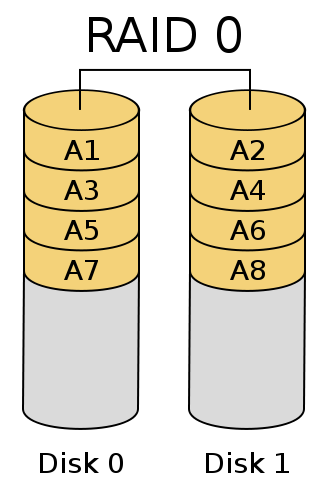
\includegraphics[width=0.6\textwidth]{img/RAID0}
  \end{columns}
  
\end{frame}

\begin{frame}
  \frametitle{RAID 1}
  \begin{columns}
    \column{0.50\textwidth}
    \begin{itemize}
    \item También llamado \emph{mirror}
    \item Se copian los mismos datos en todas las unidades
    \item No hay datos de paridad
    \item Baja el rendimiento
    \item Unidades mínimas: 2
    \item Tolerancia a fallos: n-1
    \end{itemize}
    \column{0.50\textwidth}
    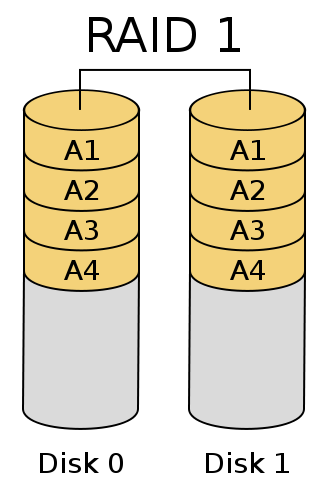
\includegraphics[width=0.6\textwidth]{img/RAID1}
  \end{columns}
  
\end{frame}

\begin{frame}
  \frametitle{RAID 4}
  \begin{columns}
    \column{0.50\textwidth}
    \begin{itemize}
    \item Se reparten los datos entre todas las unidades menos una
    \item Se utiliza una unidad para los datos de paridad
    \item Unidades mínimas: 3
    \item Tolerancia a fallos: 1
    \item Descartado en favor de RAID 5
    \end{itemize}
    \column{0.50\textwidth}
    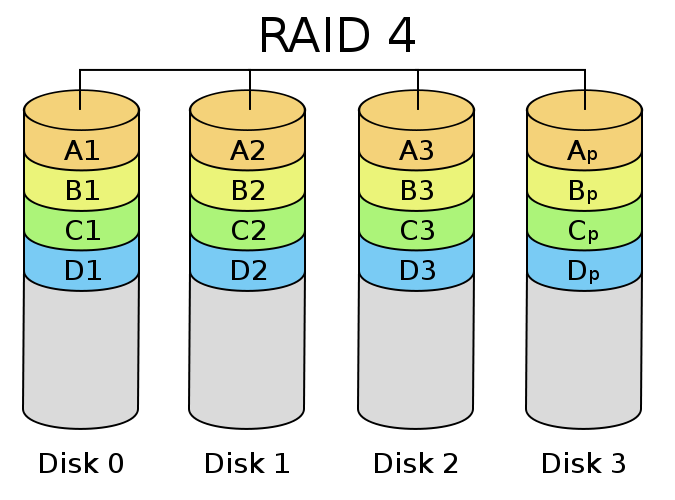
\includegraphics[width=\textwidth]{img/RAID4}
  \end{columns}
  
\end{frame}

\begin{frame}
  \frametitle{RAID 5}
  \begin{columns}
    \column{0.50\textwidth}
    \begin{itemize}
    \item Similar a RAID 4, pero se reparten los datos de paridad
      entre todas las unidades
    \item Alto rendimiento
    \item Unidades mínimas: 3
    \item Tolerancia a fallos: 1
    \end{itemize}
    \column{0.50\textwidth}
    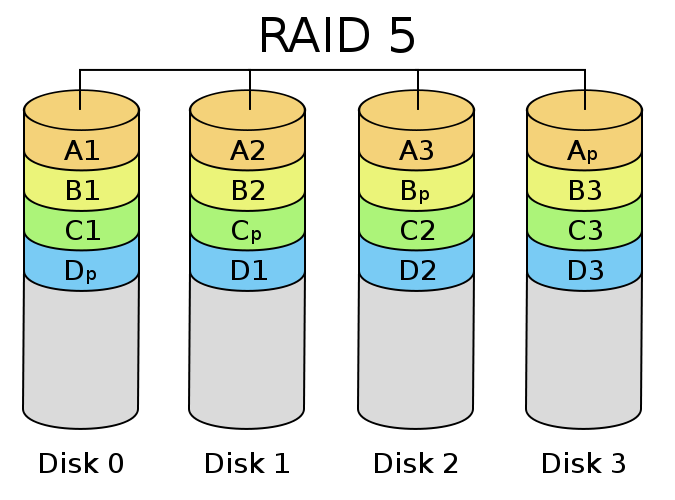
\includegraphics[width=\textwidth]{img/RAID5}
  \end{columns}
  
\end{frame}

\begin{frame}
  \frametitle{RAID 6}
  \begin{columns}
    \column{0.50\textwidth}
    \begin{itemize}
    \item Extensión de RAID 5
    \item Dos bloques de paridad repartidos en las unidades
    \item Peor rendimiento que RAID 5
    \item Mayor tolerancia a fallos que RAID 5
    \item Unidades mínimas: 4
    \item Tolerancia a fallos: 2
    \end{itemize}
    \column{0.50\textwidth}
    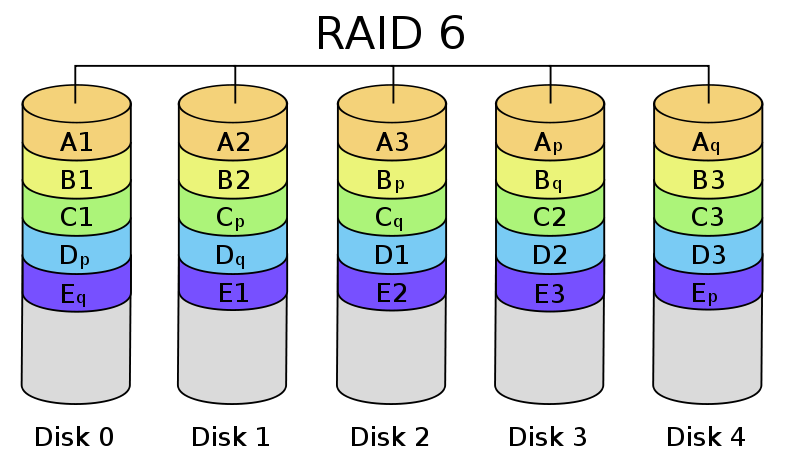
\includegraphics[width=\textwidth]{img/RAID6}
  \end{columns}
  
\end{frame}

\begin{frame}
  \frametitle{Disco de reserva}
  \begin{itemize}
  \item En la mayoría de las configuraciones RAID, una vez que se
    produce un fallo, los datos no son accesibles hasta que se ha
    sustituido el disco y se ha restaurado su contenido.
  \item Es recomendable utilizar un disco de reserva o \emph{hot
      spare}, como suplente de la unidad de disco que tenga un fallo.
  \item Este disco permanece inactivo hasta que falla un disco del
    RAID, momento en el que se activa y lo sustituye.
  \item Utilizando un \emph{hot spare} se reduce mucho el tiempo de
    recuperación de los datos
  \end{itemize}
\end{frame}

\end{document}